Simulation results when using both controllers with $K_\omega=500$ and $K_\psi=5$. 
\begin{figure}[H]
    \centering
    
    \begin{subfigure}[b]{6cm}
        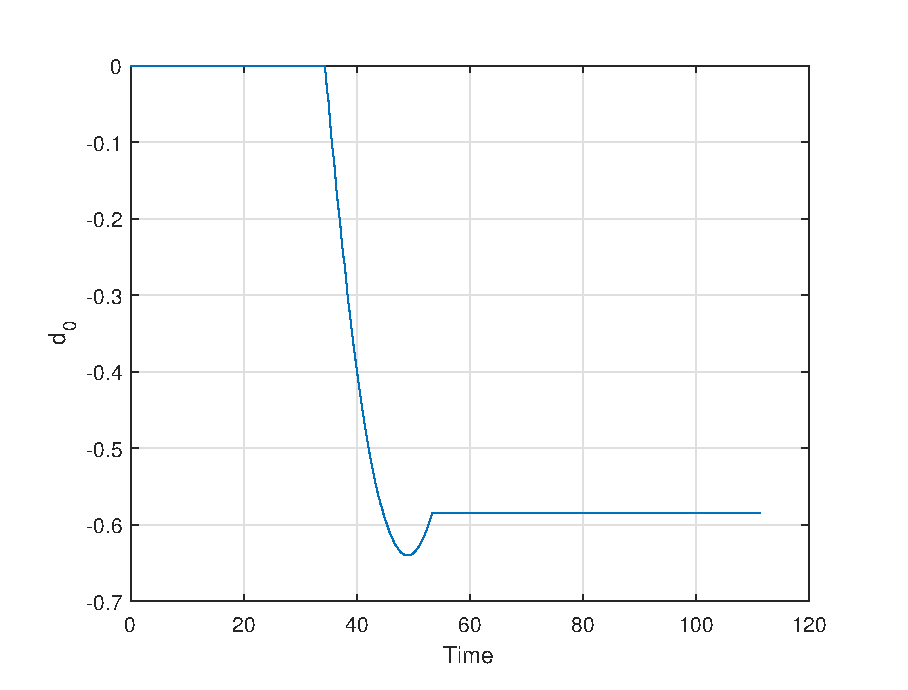
\includegraphics[width=\textwidth]{task_9_500_d0_initial_000_Goal_2090.eps}
        \caption{Initial position: (0,0) 0 degrees}
        \label{fig:d0002090}
    \end{subfigure}
    \begin{subfigure}[b]{6cm}
        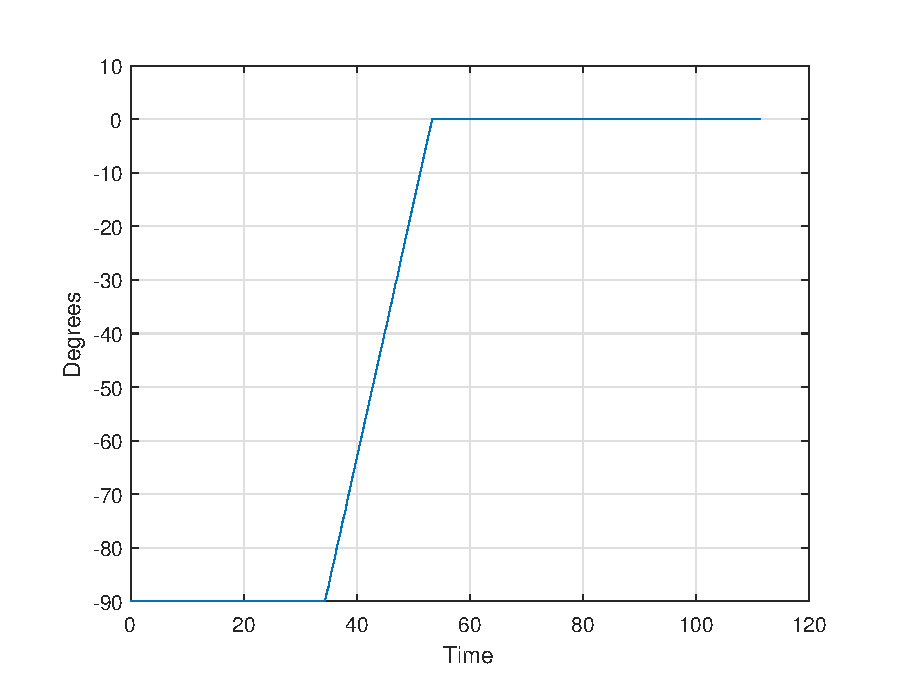
\includegraphics[width=\textwidth]{task_9_500_deg_initial_000_Goal_2090.eps}
        \caption{Initial position: (0,0) 0 degrees}
        \label{fig:deg0002090}
    \end{subfigure}
   
   
    \begin{subfigure}[b]{6cm}
        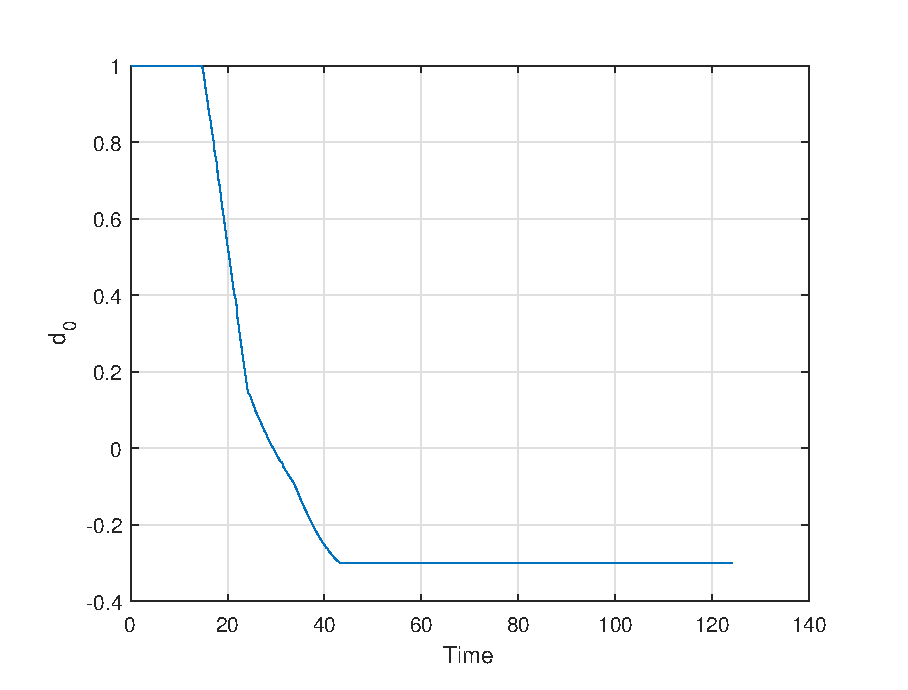
\includegraphics[width=\textwidth]{task_9_500_d0_initial_11180_Goal_2090.eps}
        \caption{Initial position: (1,1) 180 degrees}
        \label{fig:d0111802090}
    \end{subfigure}
     \begin{subfigure}[b]{6cm}
        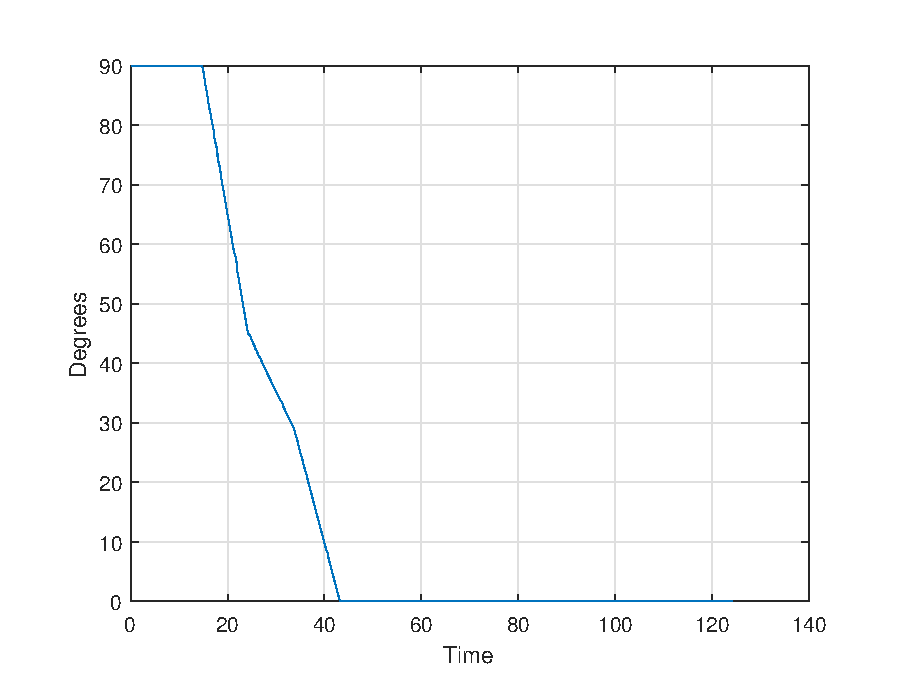
\includegraphics[width=\textwidth]{task_9_500_deg_initial_11180_Goal_2090.eps}
        \caption{Initial position: (1,1) 180 degrees}
        \label{fig:deg111802090}
    \end{subfigure}
    \caption{Goal: (2,0) 90 degrees}\label{fig:2090}
\end{figure}



\begin{figure}[H]
    \centering
    \begin{subfigure}[b]{6cm}
        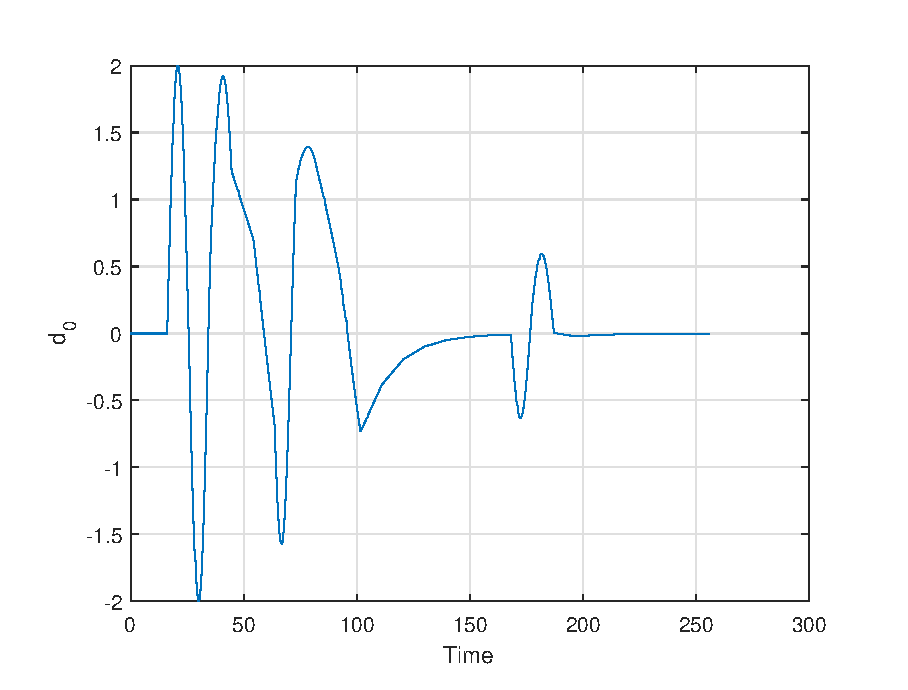
\includegraphics[width=\textwidth]{task_9_500_d0_initial_000_Goal_02180.eps}
        \caption{Initial position: (0,0) 0 degrees}
        \label{fig:d0009002180}
    \end{subfigure}
    \begin{subfigure}[b]{6cm}
        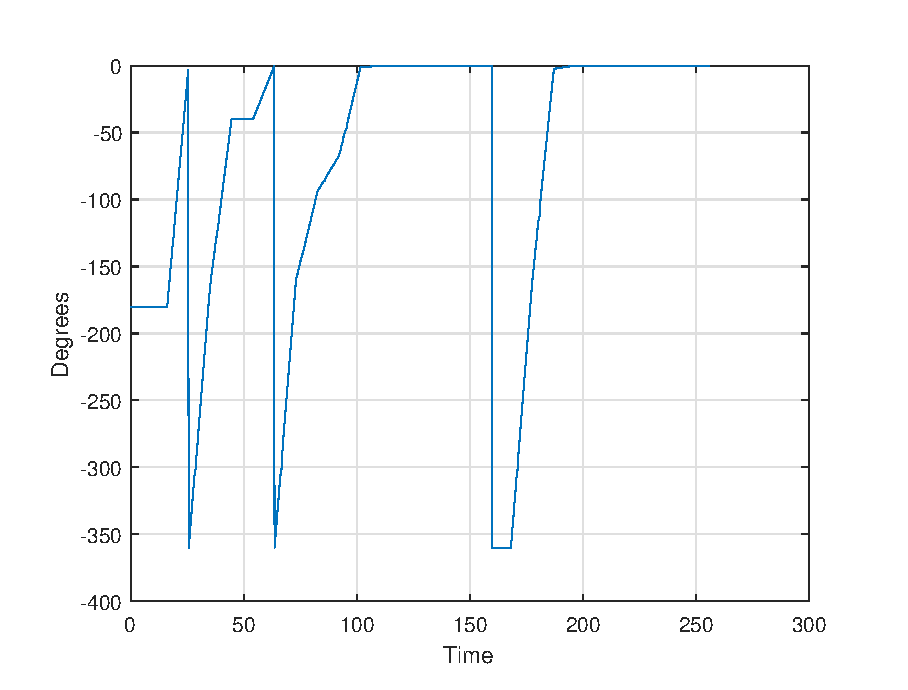
\includegraphics[width=\textwidth]{task_9_500_deg_initial_000_Goal_02180.eps}
        \caption{Initial position: (0,0) 0 degrees}
        \label{fig:deg009002180}
    \end{subfigure}
   
   
    \begin{subfigure}[b]{6cm}
        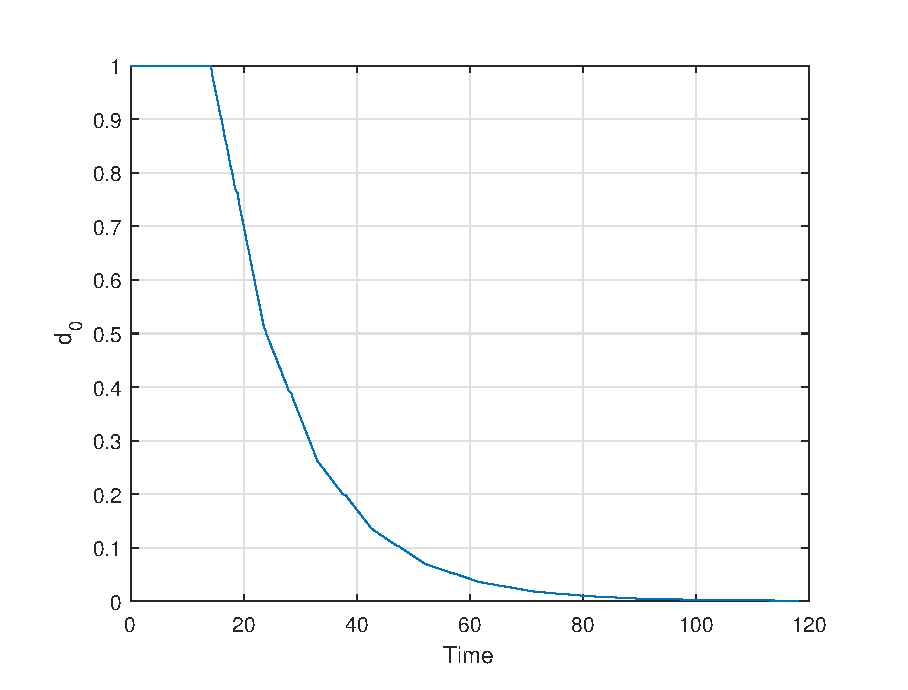
\includegraphics[width=\textwidth]{task_9_500_d0_initial_11180_Goal_02180.eps}
        \caption{Initial position: (1,1) 180 degrees}
        \label{fig:d01118002180}
    \end{subfigure}
     \begin{subfigure}[b]{6cm}
        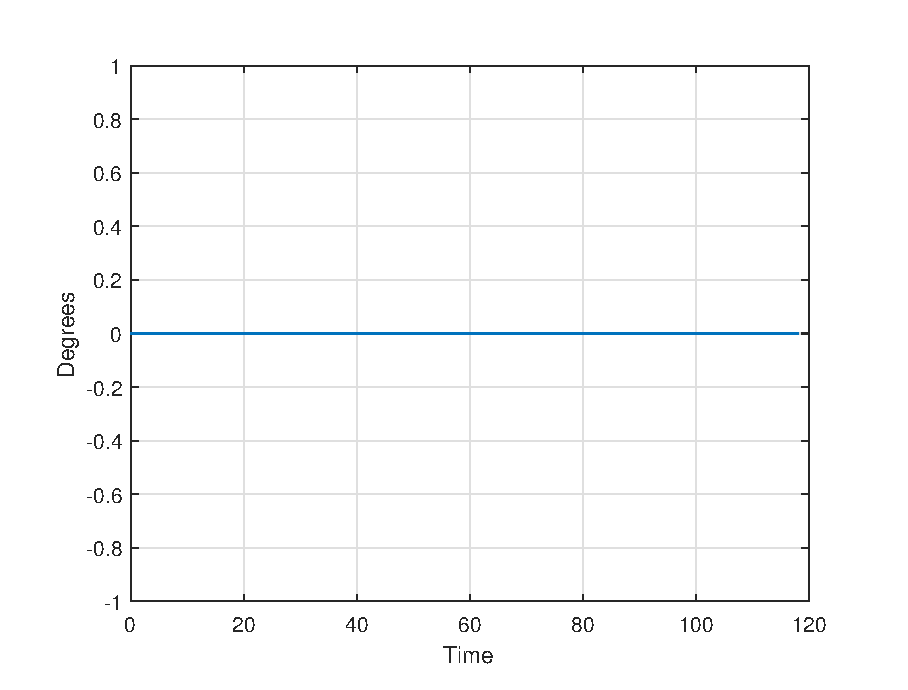
\includegraphics[width=\textwidth]{task_9_500_deg_initial_11180_Goal_02180.eps}
        \caption{Initial position: (1,1) 180 degrees}
        \label{fig:deg1118002180}
    \end{subfigure}
    \caption{Shows $d_0$ and $\theta-\theta^R$. Goal: (0,2) 180 degrees}
\end{figure}

\begin{figure}[H]
    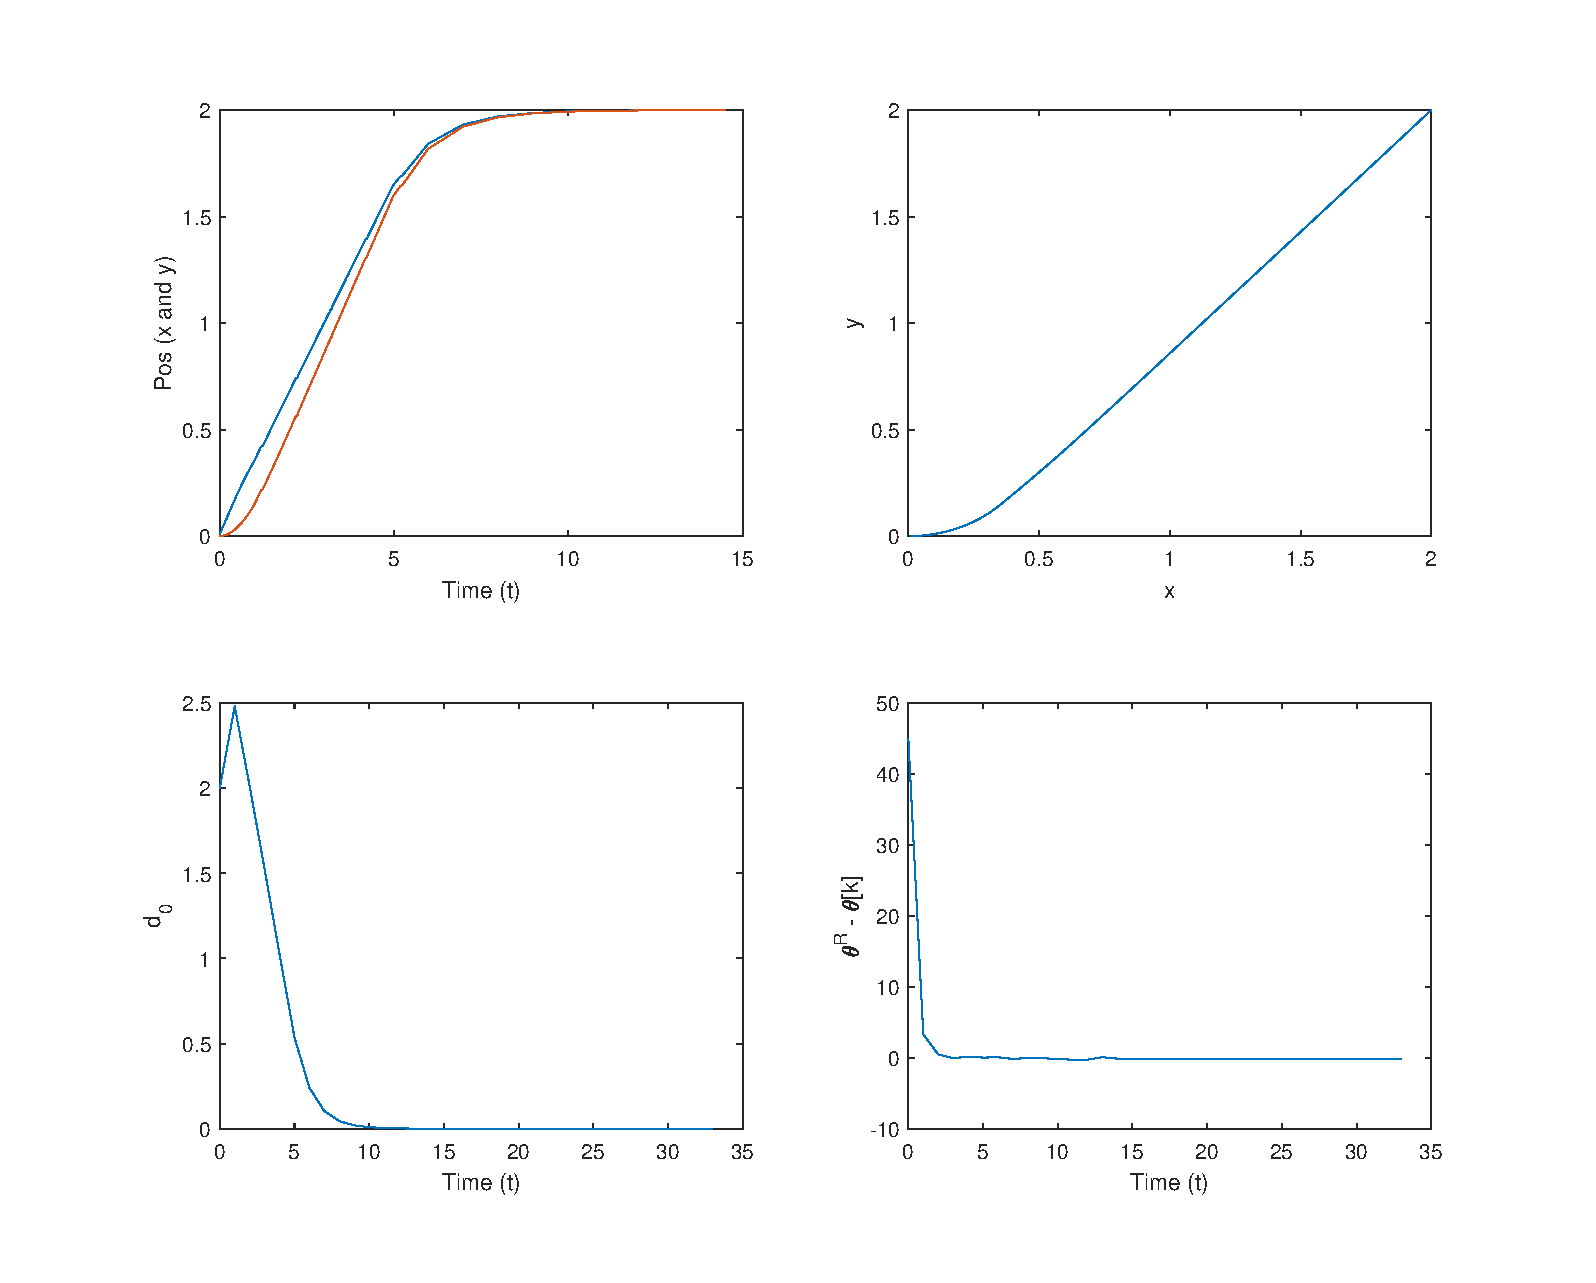
\includegraphics[width=\textwidth]{figs/perf-d0-theta.eps}
    \caption{Simulation of the combined $\Delta \theta$ and the $d_0$  controller going from $(0, 0)$ to $(2, 2)$ with $K_\omega= \frac{180}{R \pi}$ and $K_\psi= \frac{L}{R}$  }\label{fig:02180}
\end{figure}

In the first situations, the controller works fairly good. It can approach the target position first. Then it rotates toward the reference direction as it moving towards the target position simultaneously. The robot finishes the leftover rotation when it reach the target position. This is completely different from the situation when the reference direction differs greatly from the direction towards the target position. 

From the plots, some very oscillating behaviours can be observed when the desired direction and movement direction differs greatly. In these situations, the robot basically stops several times and rotates toward the desired direction and rotate back during the movement toward the desired location. This is undesired since it takes much time and create instability but does not bring any benefit. So it is not a good idea to enable both of these controller simultaneously. 